\subsection{Porovnanie prístupov}
Nakoniec by sme mali porovnať jednotlivé prístupy optimalizácie prevádzky zariadenia medzi sebou a zhodnotiť ich výhody aj nevýhody. Na tento účel sme sa rozhodli využiť iteračný prístup k optimalizácii. Experiment sme nastavili podobne ako v predchádzajúcich častiach s tým rozdielom, že v tomto prípade sme experiment vykonali pre 50 rôznych realizácií šumu merania a výsledné riešenia spriemerovali. Rozptyl šumu merania pre koncentráciu biomasy sme nastavili rovný $ W_{x} = 0.03\si{\gram\per\liter} $ a pre koncentráciu substrátu $ W_{s} = 0.025\si{\gram\per\liter} $. Pri schéme úpravy modifikátora sme zvolili váhový koeficient $ c = 0.8 $ a pri identifikácii FIR modelu sme nastavili chybu modelu rovnú dvojnásobku rozptylu šumu merania $ \delta_{s} = 0.05\si{\gram\per\liter} $. Pri dvojkrokovej optimalizácii sme zvolili počiatočný nástrel odhadovaných parametrov nasledovne $ \mu_{m} = 0.5\si{\per\hour}, K_{M} = 1.0\si{\gram\per\liter}, K_{I} = 50.0\si{\gram\per\liter} $. 

Výsledok tohto porovnania môžeme vidieť na Obr. \ref{fig:opt_approaches_comparison} resp. na Obr. \ref{fig:opt_approaches_comparison_zoomed}, ktoré zobrazujú priebeh výsledkov optimalizácie prevádzky zariadenia troch prístupov -- dvojkroková optimalizácia, schéma úpravy modifikátora a hybridné modelovanie -- vyjadrených ako hodnoty účelovej funkcie Monod modelu. Aby sme mohli kvantifikovať úspešnosť jednotlivých metód, zobrazili sme aj hodnotu optimálneho stavu nominálneho modelu a zariadenia.
\begin{figure}
	\centering
	\begin{subfigure}[b]{0.49\textwidth}
		\centering
		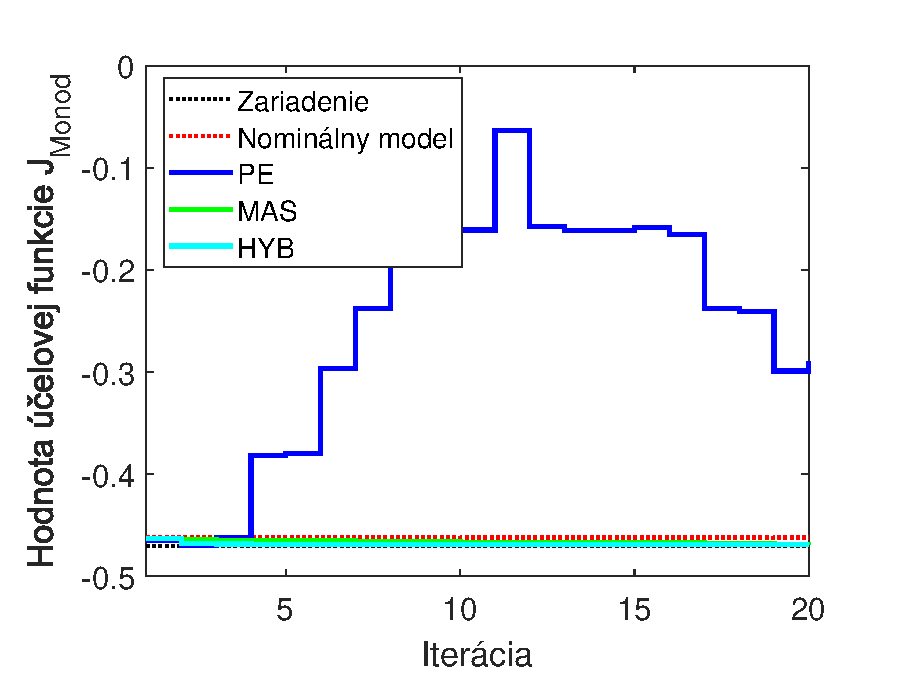
\includegraphics[width=\linewidth]{images/opt_approaches_comparison}
		\caption{Optimálne hodnoty $ D $ vyjadrené ako hodnota účelovej funkcie Monod modelu (zariadenia).}
		\label{fig:opt_approaches_comparison}
	\end{subfigure}
	\hfill
	\begin{subfigure}[b]{0.49\textwidth}
		\centering
		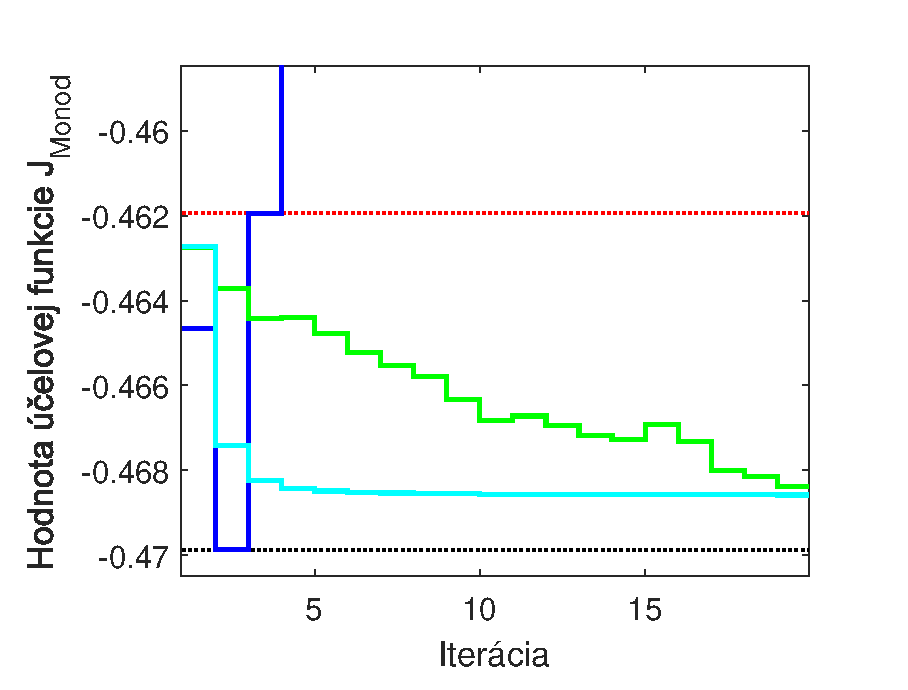
\includegraphics[width=\linewidth]{images/opt_approaches_comparison_zoomed}
		\caption{Záber z blízka. \newline \newline}
		\label{fig:opt_approaches_comparison_zoomed}
	\end{subfigure}
	\caption{Porovnanie priemerných výsledkov optimalizácie prevádzky zariadenia jednotlivých prístupov pri rôznych realizáciách šumu merania s rozptylom $ W_{x} = 0.03\si{\gram\per\liter} $ a $ W_{s} = 0.025\si{\gram\per\liter} $. Označenie \aps{PE} reprezentuje dvojkrokovú optimalizáciu, \aps{MAS} schéma úpravy modifikátora, \aps{HYB} hybridné modelovanie.}
	\label{fig:method_comparison_bigNoise}
\end{figure}

Dvojkroková optimalizácia sa vo väčšine prípadov už v druhej iterácii dostala do blízkosti optima zariadenia, ale v ďalších iteráciách sa od neho výrazne vzdialila. To je úplne odlišné správanie od toho, čo sme uviedli v predchádzajúcich výsledkoch dvojkrokovej optimalizácie, pretože tam boli uvedené výsledky iba pre jednu realizáciu šumu, na ktorých sme demonštrovali iné aspekty optimalizácie ako modularita Haldane modelu a pod. Tu však môžeme vidieť, že vo väčšine prípadov nás dvojkroková optimalizácia nedokáže priviesť do optimálneho ustáleného stavu zariadenia. Dôvod je nasledovný. V prípade, že máme k dispozícii iba male množstvo údajov, tak odhad parametrov je relatívne nepresný, čo náhodou vedie ku kombinácii parametrov nominálneho modelu, ktorého optimálny ustálený stav sa zhoduje so zariadením. Ale so zvyšujúcim sa počtom údajov nám rastie aj presnosť odhadu a interval možných hodnôt parametrov sa zmenšuje. Výsledkom potom môže byť nominálny model, ktorého účelová funkcia má taký priebeh, že spôsobuje problémy pri samotnej optimalizácii (najmä pri veľkých hodnotách $ K_I $, rádovo $ 10^{10} $ a pod.). Najhoršie na tom je, že výsledné hodnoty rýchlosti riedenia získané optimalizáciou vedú náš systém do stavu vymytia.

Teoreticky, najlepšie by si s problematikou optimalizácie prevádzky zariadenia na základe nepresného mechanické modelu mala poradiť schéma úpravy modifikátora, pretože ako jediná metóda nás dokáže dostať do skutočného optima zariadenia. Toto by sa týkalo situácie, keby výstupy zo systému neboli zaťažené chybou merania. V opačnom prípade už nemáme zabezpečenú konvergenciu. Ako môžeme vidieť na Obr. \ref{fig:opt_approaches_comparison_zoomed}, tak po 20 iteráciách sme sa v priemere dostali do blízkeho okolia optimálneho režimu zariadenia. Jasnou nevýhodou tejto metódy je, že vo väčšine prípadov je konvergencia veľmi pomalá a to môže byť veľký problém, ak jedna iterácia trvá hodiny alebo dni ako v našom prípade. Ďalšou nevýhodou je, že potrebujeme údaje o ustálenom stave koncentrácie biomasy a tá sa bežne ani nemeria, a keď aj áno, tak s veľkým rozptylom chyby merania. Avšak, táto metóda má potenciál byť silným nástrojom pri riešení optimalizácie zariadenia, ale nastavenie tejto metódy tak, aby sme zabezpečili aspoň ako takú efektivitu, je veľmi náročné a pravdepodobne si vyžaduje množstvo ďalších úprav.

V prechádzajúcej časti sme uviedli, že iteračná metóda v spojení s hybridným modelovaním nie sú najvhodnejším adeptom na hľadanie optimálneho ustáleného stavu zariadenia. A to z dôvodu, že nedokáže skonvergovať ku skutočnému optimu zariadenia, ale dostane sa iba do jeho blízkeho okolia. Na druhej strane, ak si porovnáme jednotlivé priebehy optimalizačného procesu, viď Obr. \ref{fig:opt_approaches_comparison_zoomed}, je zrejmé, že táto metóda si vo väčšine prípadov vedie najlepšie, aj napriek spomenutému nedostatku. Najväčším rozdielom oproti schéme úpravy modifikátora je v rýchlosti konvergencie. Ak zhodneme na tom, že v priemere sa dostali do rovnakej vzdialenosti od optima, tak zatiaľ čo schéme úpravy modifikátora to trvalo 20 iterácií, čo je v prípade biochemického reaktora 1000 hodín, hybridným modelom to trvalo 5 iterácií, teda 250 hodín. Ďalšou výhodou je, že pri hybridnom modelovaní, šum merania nezohráva tak významnú úlohu, akou je pri schéme úpravy modifikátora. 